% ---------
%  Compile with "pdflatex hw0".
% --------
%!TEX TS-program = pdflatex
%!TEX encoding = UTF-8 Unicode

\documentclass[11pt]{article}
\usepackage{jeffe,handout,graphicx}
\usepackage[utf8]{inputenc}		% Allow some non-ASCII Unicode in source

% =========================================================
%   Define common stuff for solution headers
% =========================================================
\Class{CS/ECE 374}
\Semester{Spring 2023}
\Authors{1}
\AuthorOne{William Cheng}{shihuac2@illinois.edu}
%\Section{}

% =========================================================
\begin{document}

% ---------------------------------------------------------


\HomeworkHeader{10}{1}	% homework number, problem number

\begin{solution}
\begin{enumerate}[(a)]
\item Let $T$ be a local-optimum tree of $G$. It must be a spanning tree of $G$ because it starts with an arbitrary spanning tree, and during each iteration, a cycle is formed and an edge is taken from that cycle so that every vertex on that cycle is still in the tree, and every vertex not on that cycle is left unchanged, therefore $T$ still spans all vertices.

Suppose $T$ is not an MST. Let $T'$ be the unique MST of $G$. We know that there is a unique MST because all the edge weights are distinct. Then there exists some edge $e=(u, v)$ such that $e\in T'$ and $e\notin T$. Adding $e$ to $T$ will form a cycle $C=p_T(u, v)+e$. We know that each cycle identifies one unsafe edge which is the most expensive edge (from lecture slides). By definition of local-search, we know that $w(e)>w(e_i)$ for any $e_i\in p_T(u, v)$, otherwise the local-search algorithm would swap $e$ with $e_i$ until no swaps can be made. Therefore, $e$ is an unsafe edge. Since $T'$ is an MST, it must be the set of all safe edges in $G$ (from lecture slides). However, $e$ is in $T'$ and $e$ is an unsafe edge, which is a contradiction. Therefore, $T$ must be an MST.
\item Consider an optimal solution $T^*$. Since all $u\in U$ are leaves, we can remove all $u\in U$ and the incident edges in $T^*$. The rest of $T^*$ must be an MST of $V\setminus U$ because otherwise we use an MST and connect it to vertices in $U$ to form a lower cost solution. Therefore, we compute the MST of $G$ with vertices and incident edges in $U$ removed, and then add the lowest cost edge from each $u\in U$ to the MST to find the optimal solution. Following is the algorithm.
\begin{algo}
	\textsc{\textul{CheapestSpanningTree($G, U$):}}\+
\\	copy $G$ to $G'$
\\	for each vertex $u$ in $U$\+
\\	$V'\gets V'\setminus \{u\}$
\\	for each edge $e\in E'$ containing $u$\+
\\	$E'\gets E'\setminus \{e\}$\-\-
\\	$T\gets \text{MST of $G'$ using Prim's algorithm}$
\\	if Prim's algorithm reports $G$ is not connected\+
\\	return \emph{nil}\-
\\	sort the edges in $E$ in non-decreasing weight
\\	mark all vertices $u\in U$ as unvisited
\\	for each edge $uv\in E$ in non-decreasing weight\+
\\	if $v\in U$ and $u\notin U$\+
\\	swap $u,v$\-
\\	if $u\in U$ and $v\notin U$\+
\\	if $u$ is unvisited\+
\\	add $uv$ to $T$
\\	mark $u$ as visited\-\-\-
\\	if there is at least one unvisited $u\in U$\+
\\	return \emph{nil}\-
\\	return $T$
\end{algo}
The algorithm will return \emph{nil} if there is no feasible solution. Let $m=|E|$ and $n=|V|$. The time complexity for Prim's algorithm is $O(m+n\log{n})$. The time complexity for sorting the edges is $O(m\log{m})$. Therefore, the time complexity of this algorithm is $O(m\log{m}+n\log{n})$.
\end{enumerate}
\end{solution}

% ---------------------------------------------------------
\HomeworkHeader{10}{2}

\begin{solution}
\begin{enumerate}[(a)]
\item Consider the following example.
\begin{figure}[h]
  \centering
  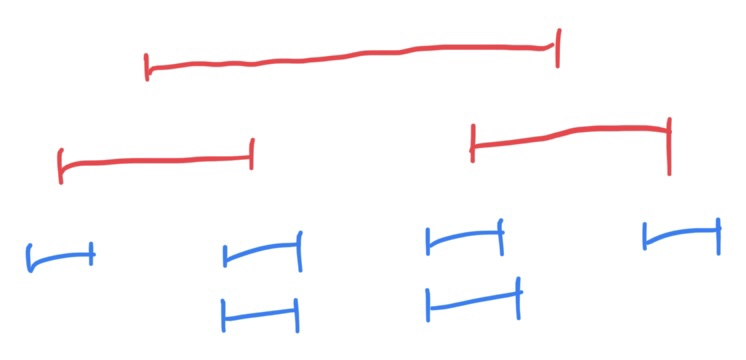
\includegraphics[width=0.5\textwidth]{hw10_2a.jpg}
\end{figure}\\
Obviously, the optimal solution is the set of the two shorter red intervals. However, if we use the algorithm described in (a), the longest red interval would first be added to the set since it covers $4$ blue intervals while the others cover $3$ each. The remaining two blue intervals would need both of the shorter red intervals to be covered. The solution would be the set of all red intervals. Therefore, the output of the algorithm in (a) is not always optimal.
\item We use the following strategy: sort $R$ and $B$ in increasing left endpoint, and iterate through $B$. Let $J_i$ be the current blue interval. We find the interval in $R$ that covers the most intervals among the intervals that cover $J_i$. Call that interval $I_i$ and add $I_i$ to the solution set. Then we remove all red intervals that cover $J_i$, remove all blue intervals that are covered by $I_i$, and recurse. Following is the pseudocode for the algorithm.
\begin{algo}
	\textsc{\textul{MinSetOfRedIntervals($R, B$):}}\+
\\	sort $R, B$ in increasing left end point order
\\	add a sentinel $I_s$ that doesn't cover any blue intervals to the end of $R$
\\	$A\gets \textsc{FindOneAndRecurse($R, B$)}$
\\	return $A$\-
\\
\\	\textsc{\textul{FindOneAndRecurse($R[1...n], B[1...m]$):}}\+
\\	if $m=0$\+
\\	return \{\,\}\-
\\	$J_1\gets B[1]$
\\	$\emph{bestRed}\gets \emph{None}$
\\	for each $I_i$ in $R$\+
\\	if $I_i$ does not cover $J_1$ and $\emph{bestRed}\ne \emph{None}$\+
\\	remove intervals up to (not including) $I_i$ in $R$
\\	remove intervals covered by \emph{bestRed} in $B$
\\	$A'\gets \textsc{FindOneAndRecurse($R, B$)}$
\\	if $A'=\text{"No valid solution"}$\+
\\	return \text{"No valid solution"}\-
\\	return $\{\emph{bestRed}\}\cup A'$\-
\\	else if $I_i$ covers $J_1$ and $b(I_i)>b(\emph{bestRed})$\,\,\,\,\,\,\,\,\,// $b(\emph{None})=-\infty$\+
\\	$\emph{bestRed}\gets I_i$\-\-
\\	return "No valid solution"\-

\end{algo}

\emph{\textbf{Time complexity:}} Sorting $R, B$ takes $O(n\log{n}+m\log{m})$ time. Then we essentially visit every interval exactly once with constant-time operations, which takes $O(n+m)$ time. Therefore, the time complexity of this algorithm is $O(n\log{n}+m\log{m})=O(n\log{(n+m)}+m\log{(n+m)})=O((n+m)\log{(n+m)})$.

\emph{\textbf{Correctness:}} To prove the correctness of this algorithm, we first prove that the first interval added to the solution by this algorithm is included in some optimal solution, then use induction to prove the general case.

\emph{\textbf{Claim:}} Let $I_i$ be the red interval added to the solution set (\emph{bestRed} in pseudocode) using the above algorithm. Let $A^o$ be an optimal solution. Then either $I_i\in A^o$, or $I_i$ can be swapped with a single interval in $A^o$ without invalidating the solution.

\emph{\textbf{Proof:}} Let $I_l$ be the interval with the smallest left endpoint in $A^o$. Let $J_l$ be the blue interval with the smallest left endpoint. Then $I_l$ must cover $J_l$, otherwise either $I_l$ covers nothing or $J_l$ is covered by a red interval with a smaller left endpoint than $I_l$, both of which are not possible. Then we can swap $I_l$ with $I_i$ in $A^o$ and still have a valid solution set, since $I_i$ covers $J_l$ and $I_i$ covers the largest number of intervals among all the red intervals covering $J_l$. The swap does not increase the size of $A^o$, therefore it is still an optimal solution.

\emph{\textbf{Base cases:}} When $m=0$ and $n\ge 0$, the algorithm trivially returns an empty set since there is no blue interval to cover. Note that the empty set is also a valid solution since we don't need any red intervals to cover all the blue intervals. When $m>0$ and $n=0$, there is no red interval, and the algorithm will correctly report that there is no valid solution.

\emph{\textbf{Inductive hypothesis:}} Let $n=p$ and $m=q$. Assume that the algorithm produces an optimal solution for all $n<p, m<q$.

\emph{\textbf{Inductive step:}} We use the algorithm to find the first red interval $I^o$ that is added to the solution set. We have proved that $I^o$ belongs to an optimal solution $A^o$. We observe that the set $A^o\setminus \{I^o\}$ is an optimal solution to the inputs $R'$ and $B'$ where $R'=R \setminus \{I^o\}$ and $B'=B\setminus \{J_i\mid \text{$J_i$ is covered by $I^o$}\}$. (If it is not optimal, then let the optimal solution be $A'$. We can add $I^o$ to $A'$ to cover all blue intervals, and the solution $A'\cup \{I^o\}$ will be better than $A^o$, which is a contradiction since we defined $A^o$ to be an optimal solution.)

By the inductive hypothesis, we can find the optimal solution $A'$ to inputs $R', B'$ using our algorithm since $|R'|<p$ and $|B'|<q$. Then we just add $I^o$ to $A'$ and the resulting set would be an optimal solution for inputs $R, B$. If we cannot find a valid $I^o$ or we cannot find a valid $A'$, then output that there is no valid solution.

Therefore, the algorithm always finds the optimal solution or correctly reports that there is no valid solution for all $m>0, n>0$.

\end{enumerate}
\end{solution}




\end{document}
